\chapter{Interakcja z kreowaną rzeczywistością}
\label{ch:prezentacja}
 Tworzenie różnych środowisk wirtualnych wymaga wykorzystania odpowiedniego sprzętu, zarówno pod względem tworzenie oprogramowania, jego dostarczania do klientów, wyświetlania jak i samej interakcji. W poniższym rozdziale zostaną przedstawione różne sposoby prezentacji tworzonych rzeczywistości a także sposoby na interakcję w zależności od wykorzystywanych technologii. Sposoby te zmieniały się przez lata i z biegiem czasu stawały się coraz wygodniejsze w obsłudze a także tańsze, dzięki czemu były bardziej przystępne zarówno w środowisku biznesowym jak i prywatnym. Zostaną również pokazane specjalistyczne rozwiązania które zostały przystosowane wyłącznie dla biznesu. Poprzez współpracę twórców bezpośrednio z odbiorcami są oni w stanie lepiej przystosować tworzone produkty. Oprócz tradycyjnych metod reagowania na wydarzenia w świecie wirtualnym zostaną zaprezentowane nietypowe prototypy urządzeń które są zazwyczaj w fazie rozwoju, jednak spełniają bardzo specyficzne funkcje, które do tej pory są osiągane w bardzo nienaturalny sposób psując tym samym wrażenia świata wirtualnego. To właśnie jest powodem dla których firmy te starają się wyprzedzić konkurencje i zdobyć tym samym rynek w kolejnym segmencie imitacji zmysłów oraz wzajemnej zależności człowieka z sztucznym światem. 
\section{Prezentacja tworzonej rzeczywistości}
\label{sec:okulary}
	Pierwszym rodzajem rzeczywistości która zostanie opisana jest wirtualna rzeczywistość. Jest to spowodowane faktem że to właśnie od tego rodzaju kreowanego świata wszystko się rozpoczęło. W celu wyświetlania obrazu wykorzystywane są tak zwane HMD (z ang. Head Mounted Display), czyli specjalne gogle które zakładane są na głowę. Dzięki kompletnemu odizolowaniu światła ze świata zewnętrznego, mogą wyświetlać na wbudowanych ekranach zawartość świata wirtualnego, dzięki czemu osiągają pełną uwagę użytkownika - świat rzeczywisty nie wpływa na doznania podczas korzystania z tego sprzętu. Gogle te używane w obecnych czasach mają swoje początki wraz z pierwszą maszyną uznawaną jako maszynę VR - Sensorame. Twórca tego urządzenia jako pierwszy opatentował w 1960 roku pomysł na urządzenie które przypomina to co obecnie nazywamy HMD, jednak znacznie bardziej rozbudowane włączając w to zmysły takie jak na przykład węch. Niestety patent ten nie został zmaterializowany za jego życia. Pierwszym prawdziwym zbudowanym urządzeniem które spełniało rolę gogli był potocznie nazywany ``miecz damoklesa". Urządzenie to jednak było ciężkie i nieporęczne, do tego stopnie że musiało być przymocowane do sufitu. Projekty te również nie były komercyjne. Zmiana ta prawie nastąpiła wraz z nastaniem czasów firmy Sega, która zdecydowała się na próbę wypuszczenie pierwszych gogli VR. Wykorzystali oni ekrany LCD przykryte czarnym plastikiem, zestaw słuchawkowy oraz jednostkę IMU w celu śledzenia położenia głowy. Projekt jednak nigdy nie został zrealizowany ponieważ jak tłumaczyli twórcy, obawiali się oni że efekty są zbyt realistyczne i ludzie mogliby się zranić w prawdziwym świecie. Prawdziwą rewolucje rozpoczął Palmer Luckey który w 2010 zaprezentował prototyp swojego urządzenia o nazwie Oculus Rift. Jego kampania finansowania społecznego zebrała 2.4 miliony dolarów a w 2014 została zakupiona przez Facebook za 2 miliardy dolarów~\cite{hd1}. Od tamtej pory powstało wiele produktów które chcą podbić rynek gogli VR, a do najpopularniejszych rozwiązań należą wspomniany Oculus Rift, HTC Vive a także gogle VR stworzone przez firmę Sony~\cite{hd2}. Udział w rynku tych urządzeń przedstawia rysunek~\ref{fig:market_hmd}. Wykres ten pokazuje że do pozostałych udziałowców urządzeń VR należy około 20\% rynku, natomaist prawie połowa należała do firmy Sony w roku 2018, jednak udział ten spadł na rzecz rosnącej popularności Oculusa. 
	\begin{figure}[h]
\centering
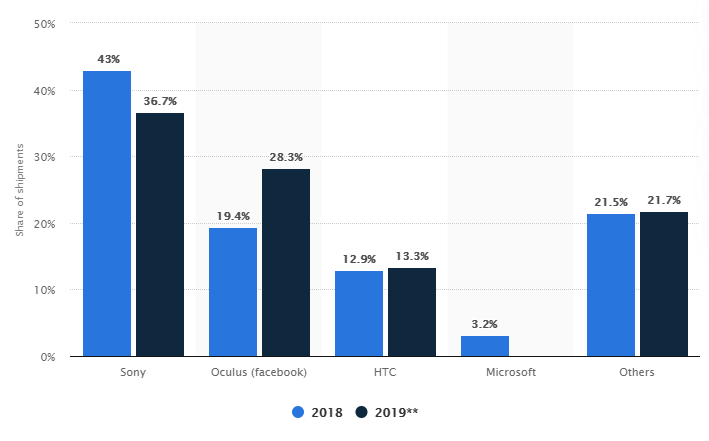
\includegraphics[width=\textwidth]{market_hmd}
\captionsource{Udział producentów w rynku urządzeń VR}{\url{https://www.statista.com/statistics/755645/global-vr-device-market-share-by-vendor/}}
\label{fig:market_hmd}
\end{figure}
 Rozwój rynku smart-fonów również przyczynił się w postępie technologii alternatywnej rzeczywistości. Firma Google stworzyła swój projekt gogli który nie zawierał ekranu, jedynie miejsce na umiejscowienie własnego telefonu. Rozwiązanie to jest tanie i łatwo dostępne jednak zapewnia jedynie podstawowe doświadczenia związane z produkcjami na ten rynek~\cite{daydream}. Świetnie natomiast sprawdziło się w przypadku rozwiązań AR. Mając do dyspozycji kamerę w telefonie, która w obecnych czasach dostarcza wysokiej jakości obrazu, oraz procesora który zapewnia całkiem dobre możliwości graficzne. Dzięki temu w czasie rzeczywistym renderowane są dla użytkownika obrazy które mogą służyć zarówno rozrywce, nauce jak i pomocy w biznesie, na przykład wśród pracowników naprawiających uszkodzone instalacje elektryczne. W tym celu jednak lepiej się sprawdzi mieszana rzeczywistość. Najbardziej znanym produktem do prezentacji MR jest produkt firmy Microsoft - Hololens. Są to specjalistyczne półprzezroczyste okulary przez które możemy obserwować świat rzeczywisty jak i wirtualny jednocześnie, a także przenosić się pomiędzy tymi światami bez żadnych problemów. Okulary te posiadają fizyczne przyciski umiejscowione wokół głowy a także zestaw kamer znajdujący się w przedniej części dzięki czemu mogą rozpoznawać otoczenie oraz powierzchnie. Obecnie istnieje już druga wersja tego urządzenia, która w porównaniu z pierwszą jest ulepszona niemal pod każdym względem. Częstym problemem podczas korzystania z pierwszej wersji było ograniczone pole widzenia. Z tego powodu wyświetlane obrazy często znikały, pomimo innych oczekiwań użytkownika. Przez lata również technologia wykrywania powierzchni się poprawiła co pozwoliło na lepsze możliwości wyświetlania obiektów w przestrzeni rzeczywistej. Dodatkowo nowa wersja została wyposażona w takie elementy jak sensor Azure Kinect, sensor pozwalający na śledzenie oczu oraz procesor ARM. W nowszej wersji, produkt ten przeznaczony jest jedynie dla biznesu i nie jest dostępny na rynku konsumenckim~\cite{holo}.
	 
  
\section{Urządzenia peryferyjne}
\label{sec:iot}
Z racji tego że do prezentacji AR wykorzystuję się najczęściej urządzenia mobilne, ekran tych urządzeń służy jako kontroler który reaguje na dotyk. W przypadku mieszanej rzeczywistości problem ten jest rozwiązywany również przez obserwację otoczenia na podstawie kamer oraz sensorów. Dzięki analizie obrazu kontrola również odbywa się w naturalny sposób poprzez gesty oraz mowę. Jedyną dziedziną w której wykorzystywane są więc dodatkowe urządzenia jest świat wirtualny, który nie bazuje wcale na świecie rzeczywistym. W tym celu należy poruszyć problem przenoszenia ruchów użytkownika do świata VR. 
Podstawową cechą wspólną rozwiązań stosowanych w goglach VR jest używanie wspomnianych wcześniej jednostek IMU (z ang. Inertial measurement unit), czyli jednostek skupiających w sobie zazwyczaj akcelerometr, żyroskop oraz magnetometr na podstawie których jest możliwe wyliczenie dokładnej orientacji urządzenia. Jednak nie da się dokładnie ustalić pozycji na podstawie tych danych, ze względu na błędy jakie generuje akcelerometr. W praktyce każdy system wykorzystuje własne rozwiązanie tego problemu, zapewniając korzyści w jednym obszarze kosztem innego - nie ma idealnego rozwiązania tego problemu. Oculus rift zdecydował się na rozwiązanie problemu położenia poprzez kamery które obserwują użytkownika. Na goglach natomiast znajduje się konstelacja diod emitujących światło podczerwone która jest wykrywana przez wspomniane kamery. Dzięki temu urządzenie jest w stanie zlokalizować użytkownika w przestrzeni a także obserwować jego ruch. Obecnie rozwiązanie to zostało przeniesione na kontrolery współpracujące z goglami. Podobną metodę działania stosuje Sony, w swoim produkcie Playstation VR. Jeszcze przed stworzeniem gogli VR, firma stworzyła kontrolery ruchu które dzięki zapalonej lampce LED były wykrywalne poprzez obserwującą je kamerę podłączoną do konsoli. Ten sam system został przeniesiony  na gogle, tworząc podświetlany produkt wykrywalny przez kamerę. Rozwiązanie to sprawiło że Sony mogło zastosować wspomniane kontrolery w swoim nowym produkcie wirtualnej rzeczywistości. Ostatnim, i dość unikalnym rozwiązaniem są wykorzystywane przez HTC Vive latarnie które w przeciwieństwie do konkurencji nie są sensorami. Są one nadajnikami które emitują światło podczerwone. Światło to z kolei jest rejestrowane przez czujniki zamontowane w zestawie VR. Dzięki temu firma ta osiągnęła wykrywanie pozycji użytkownika bez konieczności podłączania sprzętu do komputera, jednak kosztem mocowania urządzeń w pomieszczeniu które muszą być umiejscowione w przeciwległych rogach pokoju pod sufitem. W ten sposób nie tylko gogle, ale dowolny kontroler może ustalić swoją pozycję co otwiera dodatkowe możliwości dla dodatkowych urządzeń~\cite{sledzenie}. Oprócz tego fimra stworzyła specjalne odbiorniki które mogą być przymocowane do innych urządzeń i dzięki temu być śledzone w ramach tego systemu. W przeciwieństwie do rozwiązań konkurencji, do mocowania nie są używane kontrolery które normalnie trzymane są w dłoni. W przypadku HTC użytkownik może znajdować się w dowolnym miejscu w pomieszczeniu oraz sensory są znacznie mniejsze, co sprawia że komfort użytkowania jest większy, w związku z tym w dalszej części pracy posłużono się tym przykładem. System obsługuję używanie dowolnej liczby sensorów jednak przy zastosowaniu siedmiu, dwóch na stopach, dwóch na udach, jeden w pasie oraz po jednym na każdym ramieniu, w połączeniu z dwoma kontrolerami trzymanymi w dłoniach oraz goglach można mówić o pełnym śledzeniu ciała. Aplikacje takie jak chat VR w pełni je obsługują, dzięki czemu nasze ruchy w rzeczywistości są w pełni odwzorowywane~\cite{body}. Mając do dyspozycji śledzenie całego ciała, ruch w środowisku wirtualnym jest bardziej realistyczny, jednak nadal pozostają nałożone limity spowodowane przebywaniem w świecie rzeczywistym. Rozwiązaniem tego problemu zajmują się firmy których celem nie jest stworzenie systemu śledzenia ciała lecz zapewnienia mobilności użytkownikowi. W tym celu powstały specjalne, wielokierunkowe bieżnie pozwalające na dostosowanie kierunku oraz ruchu w świecie wirtualnym na podstawie zachowania w świecie rzeczywistym. Jest to odpowiedź na jeden z większych problemów stawianych przed twórcami technologii VR. Niestety rozwiązania takie jak Kat VR są nowe a co za tym idzie drogie - stanowią one jednak kolejny krok w rozwoju urządzeń zewnętrznych służących imersji w świat wirtualny~\cite{cat}. Ostatnim elementem którego brakuje w celu pełnej kontroli ciała w świecie wirtualnym jest porzucenie kontrolerów na rzecz dłoni. Ten efekt stara się osiągnąć wiele firm a pomysł został zapoczątkowany wiele lat temu. W rozdziale~\ref{ch:kontrolery} zostanie przedstawiony rozwój jaki nastąpił na rynku rękawic kontrolerów  a także zostaną opisane przykładowe rozwiązania.